\documentclass[
a4paper, 
12pt, 
]{article}

\usepackage[ngerman,english]{babel}			% Kapitel/Chapter. typographic rules
%\usepackage[english]{babel}

\usepackage[utf8]{inputenc}			% Encoding with umlauts and ß
\usepackage{graphicx}           			% include graphics
%\usepackage{lipsum}				 			% testing text as \lipsum[1-3] 			 
%\usepackage{titling}							% imports \theauthor
\usepackage{graphicx}						% include graphics
\usepackage{siunitx}							% corretct formatting of units
\usepackage[framed,numbered,autolinebreaks,useliterate]{mcode} % for matlab code

\usepackage{amsmath}            % nice equations
\usepackage{url}                			% URLs
%\usepackage{natbib}             		% author-year bibliography style
\usepackage{hyperref}           	% PDF links
%\usepackage{subfig}             	% Subfigures (a), (b), etc
%\usepackage{nomencl}            	% Nomenclature	
\usepackage{tcolorbox}
\usepackage{Systemtheorie}		 	% style with headers/footers/logo/firstpage
\fancyfoot[R]{Juri Fedjaev} 
% ----------------------------------------------------------------------------


\begin{document}
	
	\thispagestyle{firstpage} 			% use different style here (from .sty file)
	
	\section*{Neuroprothetik -- Exercise 1: Introduction}
	\subsection{Generate a Signal}
The following Matlab code generates a signal following eq. 1 and takes into account following input arguments: array of frequencies in Hz, array of amplitudes, signal duration in \textit{s}, sampling rate in Hz. 
	
\begin{align}
	f(t) = A_0 + \sum_{i=1}^{n} A_i \cdot sin(2\pi F_i \cdot t)		
\end{align}

\subsubsection{Plot the signal}
\subsubsection*{a)}
\textit{See code.}
\subsubsection*{b)}
\begin{figure}[h]
\centering
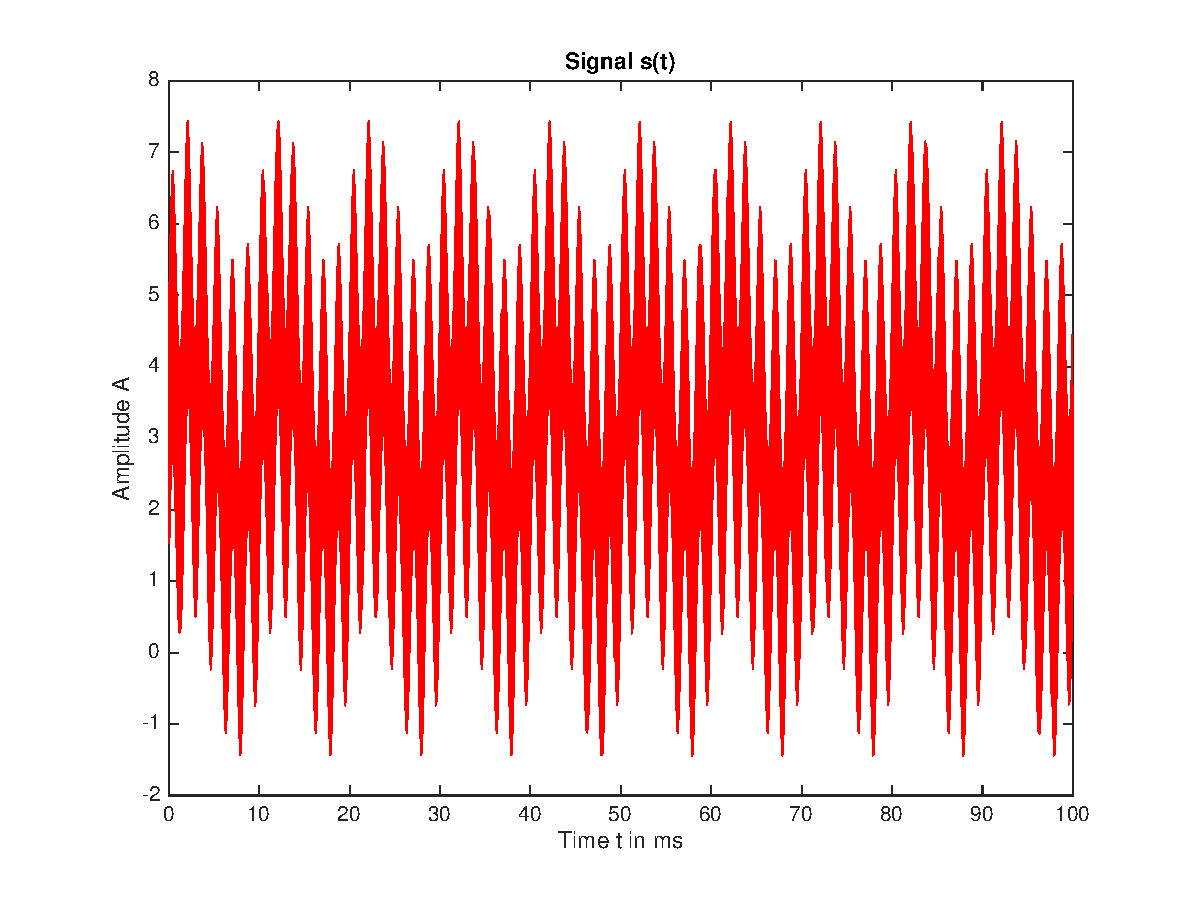
\includegraphics[width=0.7\linewidth]{Bilder/sinus_1}
\caption{Sinusoidal signal s(t) consisting of superposed frequencies 100 Hz, 600 Hz and 9 kHz with amplitudes 1, 1.5 and 2 as well as an offset of 3 at a sampling rate of 100 kHz.}
\label{fig:sinus_1}
\end{figure}


\subsection{Calculate the Spectrum}
\subsubsection*{a)}
\textit{See code.}

\subsubsection{Plot the Spectrum}
\subsubsection*{a)}
In the following plots you see the amplitude spectrum for the different sampling rates ($100$ kHz, $20$ kHz, $10$ kHz). 

\begin{figure}[h]
\centering
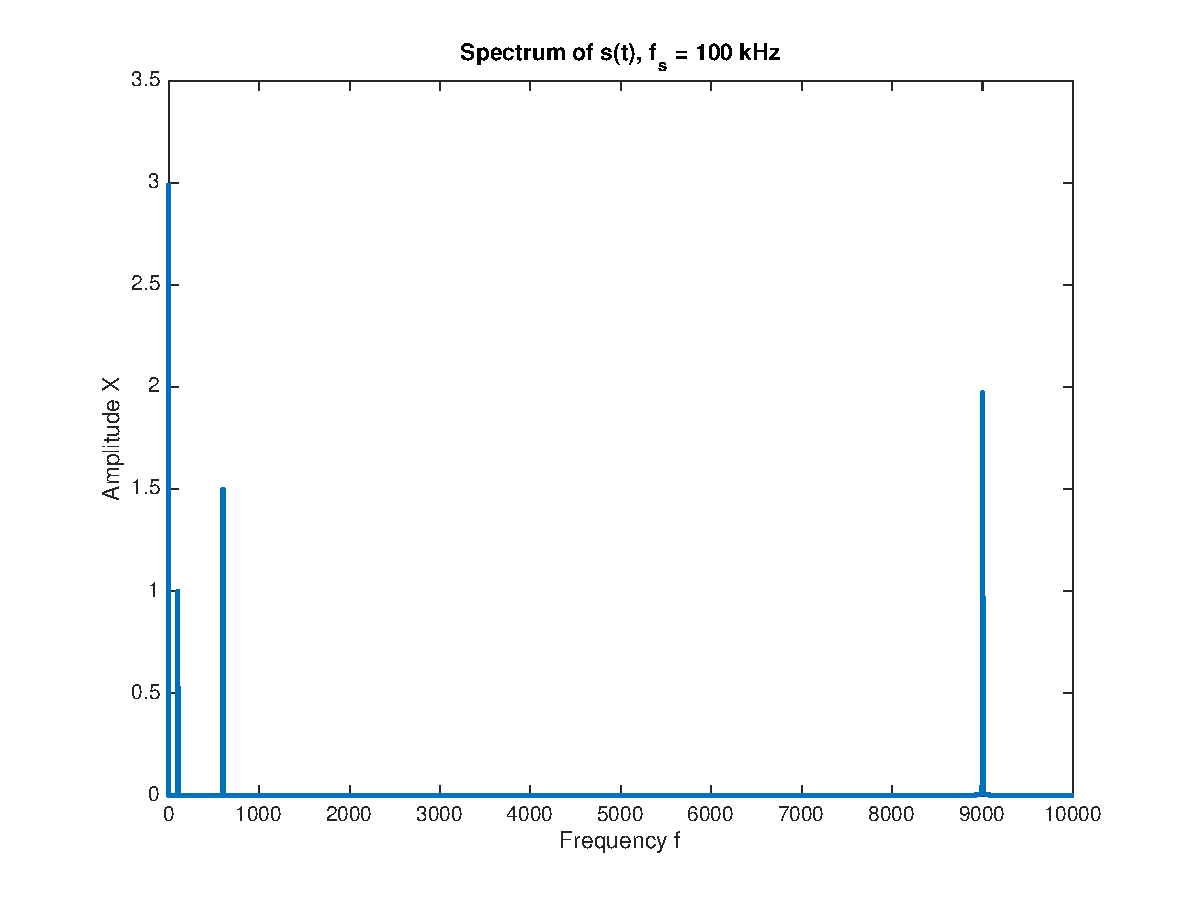
\includegraphics[width=0.7\linewidth]{Bilder/fs_1}
\caption{Amplitude spectrum for signal from section 1, with sampling rate of $100$ kHz.}
\label{fig:fs_1}
\end{figure}
\begin{figure}[h]
	\centering
	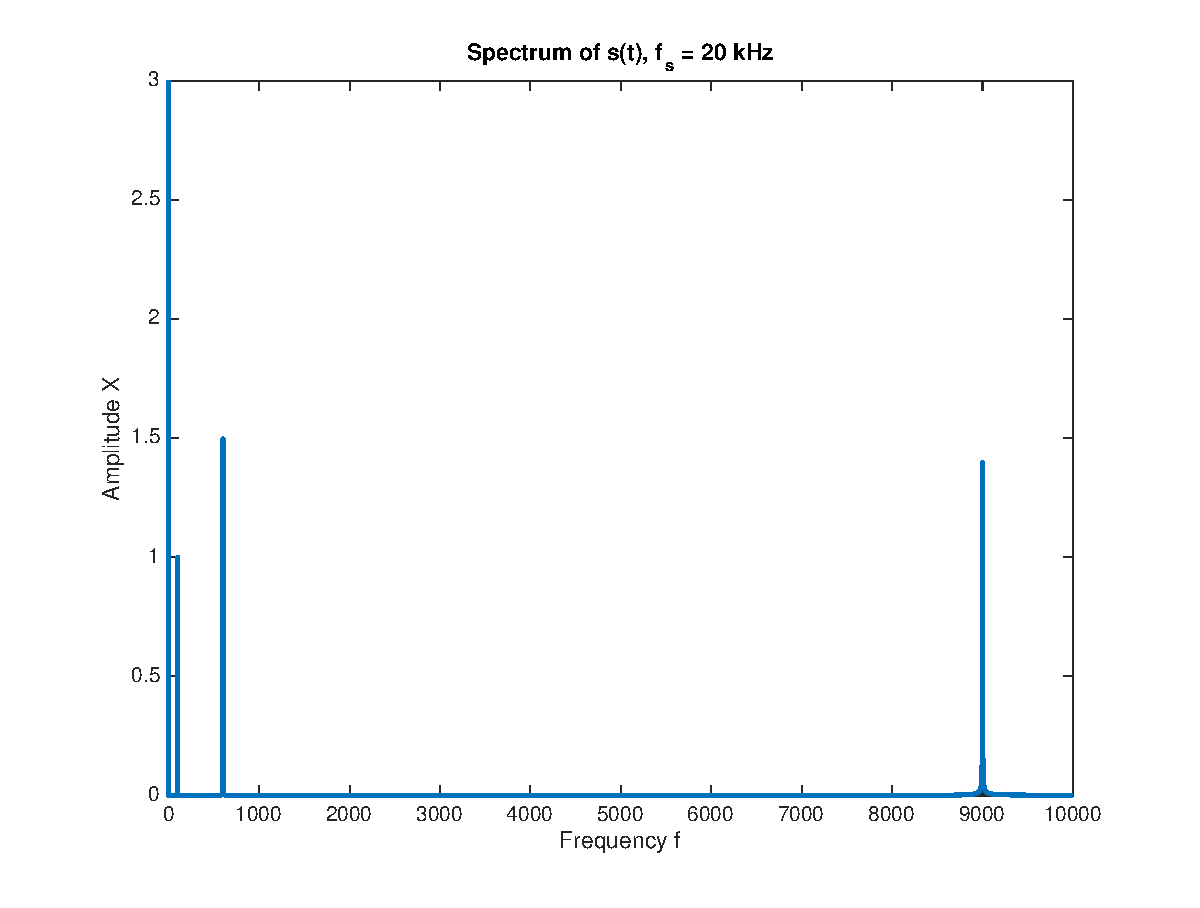
\includegraphics[width=0.7\linewidth]{Bilder/fs_2}
	\caption{Amplitude spectrum for signal from section 1, with sampling rate of $20$ kHz.}
	\label{fig:fs_1}
\end{figure}
\begin{figure}[h]
	\centering
	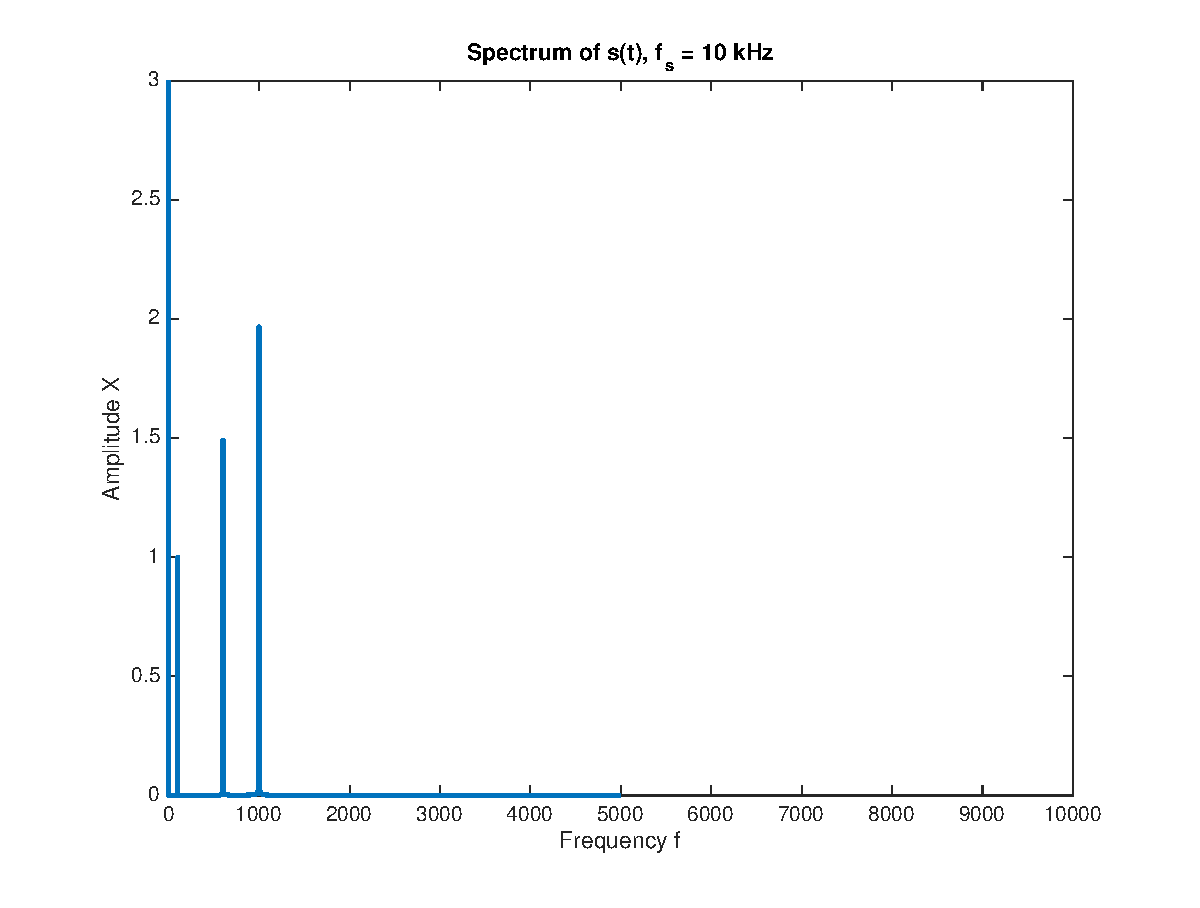
\includegraphics[width=0.7\linewidth]{Bilder/fs_3}
	\caption{Amplitude spectrum for signal from section 1, with sampling rate of $10$ kHz.}
	\label{fig:fs_1}
\end{figure}
\clearpage
\subsubsection*{b)}
For \textit{figures 1} and \textit{2}: the peak at $f = 0$ Hz is the offset with the correct amplitude $A = 3$. The next peak from the left is at $f = 100$ Hz (1$^{st}$ frequency component of the signal) with its amplitude $A = 1$. At $f=600$ Hz is the 2$^{nd}$ frequency component of the signal with $A = 1.5$. The last peak at $f=9$ kHz with an amplitude of $A=2$ is the 3$^{rd}$ frequency component of the signal.\\
For \textit{figure 3}, there is no peak at $f=9$ kHz, but an additional peak at $f=1$ kHz. That peak was shifted from the \textit{left-side spectrum}, as the FFT spectrum initially was symmetric, but only by $f_s=10$ kHz, thus resulting in $f=1$ kHz ($(10-9)~\text{kHz} = 1~\text{kHz})$, see also following paragraph).\\ 
The last spectrum (the one that was calculated based on the signal sampled at a rate of $10$ kHz) violates the Nyquist-Shannon sampling theorem. The Nyquist-Shannon sampling theorem states that for a given bandlimit $B$ of a signal, the sampling frequency $f_s$ needs to be at least twice the bandlimit:
\begin{align}
2\cdot B < f_s
\end{align}
This condition is \textbf{not fulfilled}, as the maximum frequency in signal $s(t)$ is $9$ kHz, i.e.:
\begin{align}
2\cdot 9~\text{kHz} = 18~\text{kHz} < 10~\text{kHz}
\end{align}
Therefore, aliasing artifacts occur in the amplitude spectrum of signal $s_3(t)$ between the two main spikes at $100$ Hz and $600$ Hz. The maximum admissible frequency in any signal $s(t)$ must not exceed $f_s/2$ for proper sampling and perfect reconstruction of the signal.\\\\

\begin{tcolorbox}
	\large{\textbf{Edit (11/05/2016)}: In order to avoid aliasing effects in the sampled version with a sampling rate of $f_s = 10$ kHz, it is possible to limit the band of the signal by using an \textit{anti-aliasing filter}. An anti-aliasing filter can typically be realized with a low pass filter and needs to applied to the original, analog signal $s(t)$ before sampling. That filter ideally needs to have very steep edges, so that the signal within the Nyquist limit is not distorted. The band limit of the low pass filter in the case of $f_s=10$ kHz should be $B_{LP}=5$ kHz.}
\end{tcolorbox}


	
\end{document}